\documentclass[11pt]{article}

\usepackage[a4paper]{geometry}
\geometry{left=2.0cm,right=2.0cm,top=3cm,bottom=2.5cm}
\usepackage{setspace}
\setstretch{1.5}
\usepackage{ctex}
\usepackage{amsmath,amsfonts,graphicx,amssymb,bm,amsthm}
\usepackage{algorithm,algorithmicx}
\usepackage[noend]{algpseudocode}
\usepackage{fancyhdr}
\usepackage{booktabs}
\usepackage{listings}
\usepackage{xcolor}
\lstset{
	language=Python,
	basicstyle=\ttfamily\small,
	numbers=left,
	numberstyle=\tiny,
	showstringspaces=false,
	breaklines=true,
	frame=single,    
	rulecolor=\color{black}, 
	framerule=0.6pt,     
	framesep=4pt,     
	xleftmargin=6pt,     
	backgroundcolor=\color{gray!5} 
}


\begin{document}
	\pagestyle{fancy}
	\lhead{\kaishu 中国科学院大学}
	\chead{}
	\rhead{\kaishu 2025年秋季学期\qquad 自然语言处理基础与大模型}
	
	\begin{center}
		{\LARGE \bf 课程作业1-A} 
	\end{center}
	\begin{center}
		\large\kaishu{尧祥临 202518023406038 前沿交叉科学学院}
	\end{center}
	
	\section{任务说明}
	本报告选择的是课程作业1-A,其主要任务包括:
	\begin{itemize}
		\item 收集中英文语料
		\item 计算在收集样本上英语字母和单词或汉字的概率和熵
		\item 利用收集的英文文本验证齐夫定律(Zipf’s law)
		\item 在不同样本量下探究结果差异
	\end{itemize}
	
	\section{语料获取与清洗}
	\subsection{现代与历史语料获取}
	\subsubsection{维基百科随机词条爬取}
	语料获取上,本报告为了统一在同一语言环境获取中英文语料,从而选择了维基百科(Wikipedia)作为爬取的目标,主要思路是利用了维基百科提供的随机词条功能,每次进入随机的百科词条页面之后,获取相应的词条正文内容。分别对中文维基和英文维基使用随机词条功能即可爬取到大量的语料,这样的好处是能确保爬取到的语料可以认为是正式规范的,一定程度上能反应现代英语和现代汉语的特征;但是同样也有一定的缺点,例如受百科这样的体例限制,内容主要是对人物事迹、重要事件经过以及概念的叙述,在主题上有所匮乏。
	
	完整的爬取代码如附录7.1所示。
	
	对于中文词条,爬虫脚本中访问的URL需要设置为zh.wikipedia确保随机出来的词条是中文词条,同时在最后添加variant=zh-cn确保词条文字是大陆简体;对于英文词条,只需要设置为en.wikipedia即可。经过对多个词条网页源代码的分析,发现维基百科词条的正文内容总出现\#mw-content-text > div.mw-content-ltr.mw-parser-output的路径下,所以这里我选择直接锁定这一路径,在这一路径下再获取所有位于<p>内的段落内容。这样每次爬取到的语料是来自正文而不是词条网页内其余文字内容,从而保证语料是成段落成规模的句子而不是一些杂乱的短语或者重复性的网页引导文字。
	
	\begin{lstlisting}[language=Python, label=code2.1]
if lang == 'zh':
	self.base_url = "https://zh.wikipedia.org/wiki/Special:Random?variant=zh-cn"    #加上zh-cn确保爬下来的是大陆简体中文
elif lang == 'en':
	self.base_url = "https://en.wikipedia.org/wiki/Special:Random"
	\end{lstlisting}
	
	\begin{lstlisting}[language=Python, label=code2.2]
content_div = soup.select_one('#mw-content-text > div.mw-content-ltr.mw-parser-output')	# 直接定位到该路径
paragraphs = content_div.find_all('p')
	\end{lstlisting}
	
	对于每一个词条,脚本会分别记录下三个字段,title、content和url。其中title用来记录词条的名称,例如“巴鲣 - 维基百科,自由的百科全书”;url用来记录下该词条的链接,并通过这个来保证记录下来的词条内容不会因为两次随机到了同一个词条而产生重复;最关键的content用来记录正文文本内容,在爬取过程中会在删除文本段落前后可能的空格之后将所有段落直接拼接起来,同时分别对中英文进行不同的处理:中文直接去掉文本中存在的任何空白字符,而英文则将长空格保留为一个从而至少为不同单词之间留下空格做分隔。
	
	\begin{lstlisting}[language=Python, label=code2.3]
content = ''.join([p.get_text().strip() for p in paragraphs]) 
content = ' '.join(content.split()) if self.lang == 'en' else re.sub(r'\s+', '', content)   # 分情况处理,英文需要用空格来分隔单词,中文直接可以把空白字符给去掉
	\end{lstlisting}
	
	在保存的时候,考虑到这里爬取的语料未来可能另有其他用处,所以并没有直接存储为纯文本的txt格式,而是将title、content和url作为三个字段,把每个词条写成一个json字典,最终全部爬取的文本保存为一个大的jsonl文件。对于中文和英文的语料,均爬取20000条不重复的词条,以保证文本足够充足用来进行统计分析。
	
	\subsubsection{历史语料}
	为了进一步去分析中文和英文在统计上的各种特征,本报告额外获取了一些历史语料,来探究现代汉语与现代英语同古代汉语(文言文)和古英语之间在统计上存在的差异。对于中文的历史语料本报告选择了《史记》,从某种意义上说史记的纪传体同百科的词条有一定的相似之处;对于英文的历史语料,本报告选择了莎士比亚最长的剧本《哈姆雷特》,因莎翁对于英语词汇的极大丰富与拓展。

	\subsection{清洗思路与方法}
	最终爬取到的中英文各20000条词条,但这些词条内容中存在标点符号和非中文或英文内容,所以需要对文本内容进行基本的清洗。对于中文词条,直接利用正则表达式匹配所有非中文内容并将其替换为空,最后把所有清洗后的文本拼接起来,保存为一个txt文件。而对于英文词条,则需要考虑更多。首先就是在英文词条中可能存在同样使用英文拉丁字母但并非英语词汇的情况,例如“Danke”、“Français”等,对于前者我们没办法通过简单的办法清洗出去,但是对于后者这类单词中带有非26个字母的情况可以通过匹配进行排除。其次就是连字符问题,例如“ex-wife”,作为一个完整的单词就不能直接拆为两个。最后就是需要保证单词与单词之间要有所区分,用空格进行间隔。针对这些问题,清洗英文的时候先将所有前后为空格并且内部只有26个字母或连字符组成的部分匹配下来,然后将这些部分用空格连接,最后将所有的字母都统一成小写字母,这样就方便后续对单词和字母的统计。
	\begin{lstlisting}[language=Python, label=code2.4]
self.pattern = re.compile(r'[^\u4e00-\u9fa5]')	# 匹配非中文字符
# ...... #
clean_text = self.pattern.sub('', data['content'])  # 匹配到的字符替换为空
	\end{lstlisting}
	\begin{lstlisting}[language=Python, label=code2.5]
self.pattern = re.compile(r'\b[a-zA-Z]+(?:-[a-zA-Z]+)*\b')	# 选中英文单词(包括连字符)
# ...... #
clean_text = ' '.join(self.pattern.findall(data['content']))  # 匹配到的单词用空格连接起来
clean_text = clean_text.lower()	# 统一转化为小写字母
	\end{lstlisting}
	
	\section{语料分析结果}
	以下为中英文分析结果以及与历史语料的对比分析结果,在中英文分析的时候,设置10\%、20\%一直到100\%这样十个不同样本量的情景,用来实现在不同样本量下的差异分析。其中中文直接按照汉字进行样本量划分,英文则根据单词来划分。
	
	\subsection{中文分析结果}
	中文语料共有8283290个汉字,其中共有7696不重复的汉字。对十个不同样本量情景下分别计算各个汉字的出现概率,排名前20的汉字如表\ref{tab:3.1}所示,可以看到如“的”、“年”、“为”、和“在”等排名前十一的汉字无论是哪种样本量下均稳居前排。这里“的”排名第一与现代汉语中非常喜欢在修饰词后添加“的”有关,例如“激烈的战斗”,一旦语句中大量出现形容词就会伴随着出现大量的“的”字。而“年”和“国”等词在这里排名靠前可能与语料来自于维基百科有关,这样的体裁下为了去描述某件事或人就会出现年份或国家从而提高了这两个字出现的概率。这中情况并不能直接说明这些字在现代汉语中就一定是非常高频的汉字。图\ref{fig:3.1}所示的为在10\%、20\%、50\%和全文本情景下的汉字出现概率分布图,表现为长尾分布。
	
	\begin{table}[htbp]
		\centering
		\caption{不同文本量下出现概率排名前20的汉字}
		\label{tab:3.1}
		\begin{tabular}{cc} 
			\toprule
			文本量 & 出现概率排名前20汉字 \\ 
			\midrule
			10\% & 的、年、为、在、一、国、中、是、人、于、大、月、日、 和、 有、 学、 会、 后、 以、 斯 \\
			20\% & 的、 年、 为、 在、 一、 国、 中、 是、 人、 于、 大、 和、 有、 月、 日、 学、 后、 以、 了、 会 \\
			30\% & 的、 年、 为、 在、 一、 国、 中、 是、 人、 于、 大、 和、 有、 月、 日、 以、 学、 后、 了、 会 \\
			40\% & 的、 年、 为、 在、 一、 国、 中、 是、 人、 于、 大 、和 、有 、月 、日 、以 、后 、了 、时 、学 \\
			50\% & 的、 年、 在、 为、 一、 国、 中、 是、 人、 于、 大、 和、 有、 月、 日、 以、 后、 时、 了、 学 \\
			60\% & 的、 年、 在、 为、 一 、国、 中、 是、 人、 于、 大 、和 、有 、日、 月 、以 、后、 了、 时 、斯 \\
			70\% & 的、 年、 在、 为、 一 、国 、中 、是 、人 、于、 大 、和 、有、 日 、月、 以、 后 、时、 了、 地 \\
			80\% & 的、 年、 在、 为、 一、 国、 中、 是、 人、 于、 大、 和、 有、 日、 月、 以、 后、 了、 时、 地 \\
			90\% & 的、 年、 在、 为、 一、 国 、中 、是 、人 、于 、大 、有 、和 、日 、月 、以 、后 、了 、时 、地 \\
			100\% & 的、 年、 在、 为、 一、 国、 中、 是、 人、 于、 大、 有、 和、 日、 月、 以、 后、 了、 时、 地 \\
			\bottomrule
		\end{tabular}
	\end{table}
	
	\begin{figure}[htbp] 
		\centering
		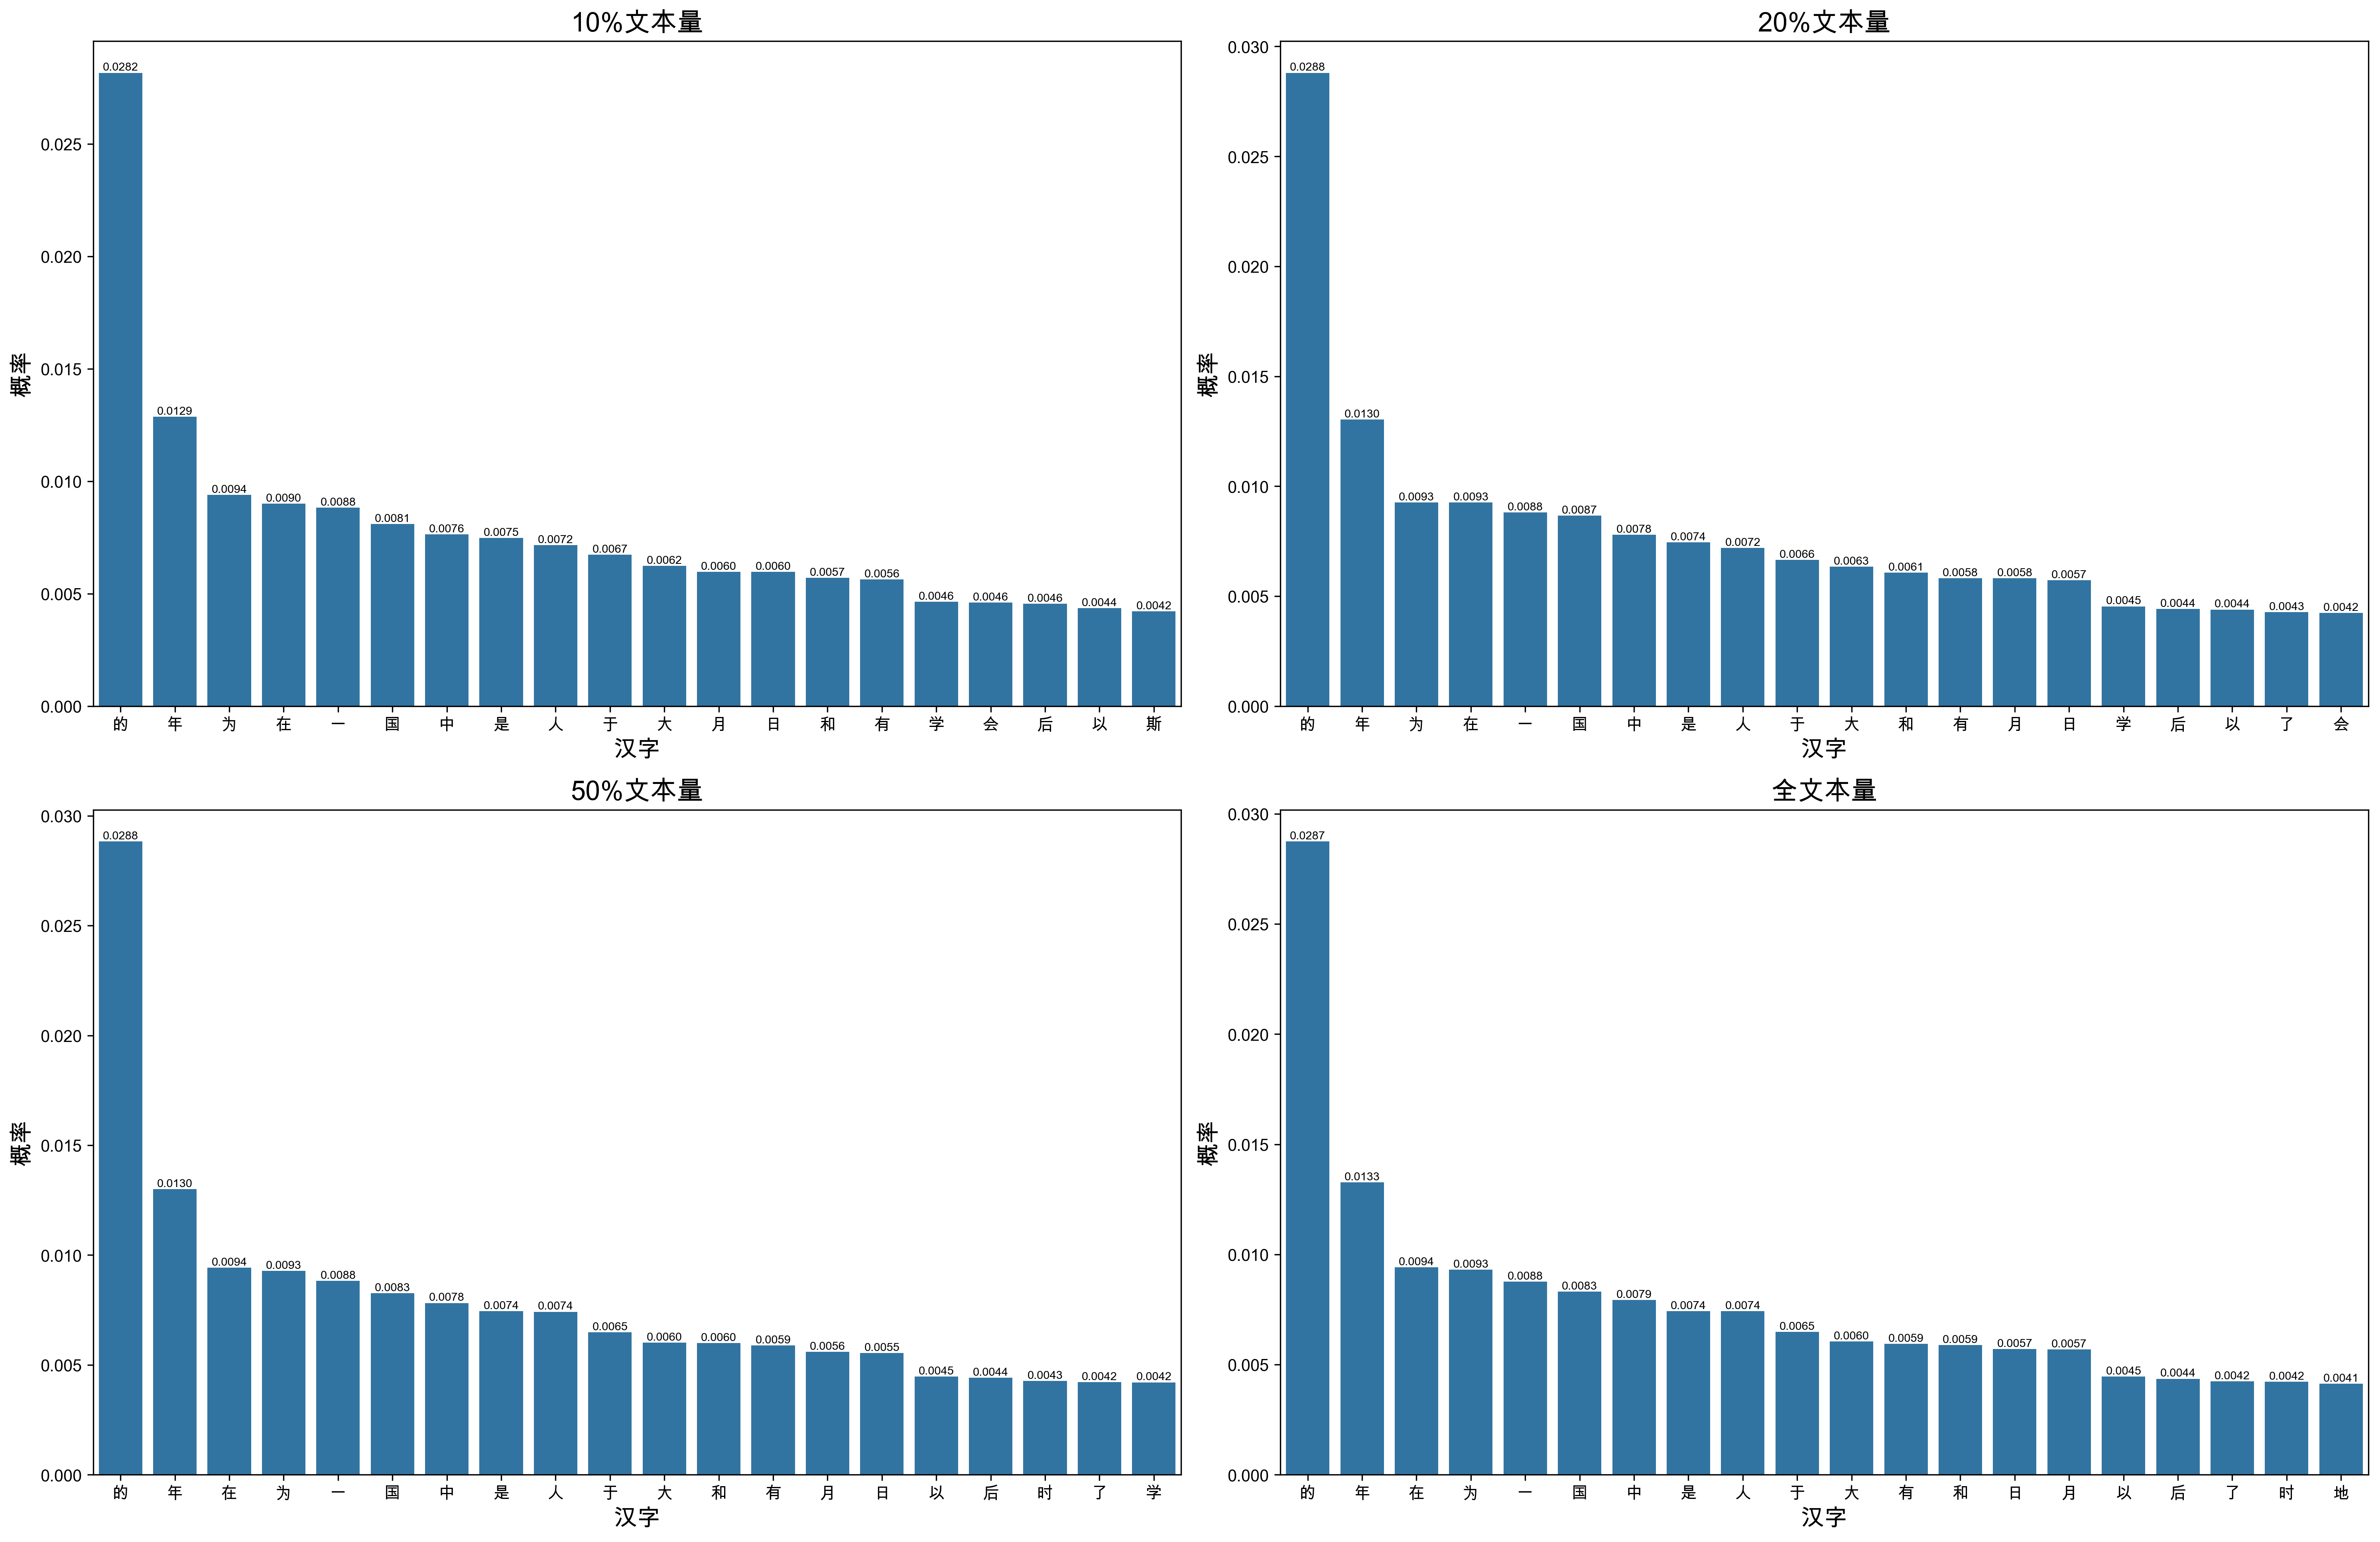
\includegraphics[width=1\textwidth]{zh_top20_char_distribution_comparison.png}
		\caption{四种文本量情景下出现概率排名前20的汉字}
		\label{fig:3.1} 
	\end{figure}
	
	对每个情景分别计算汉字熵,得到图所示的结果。可以看到中文的汉字熵表现出随着文本量的增大而增长的趋势,但总体变化幅度并不大,全文本情景下汉字熵为9.8314,这一结果与课件上所展示的9.71的汉字熵数值上接近,一定程度上证明了结果的准确性。在全文本中,由于共有7696个不重复的汉字,所以在等概率条件下汉字熵应为$\log_27696 \approx 12.9099$,而实际的熵比这个要小,这与前文中所展现的汉字概率分布情况相匹配。
	
	\begin{figure}
		\centering
		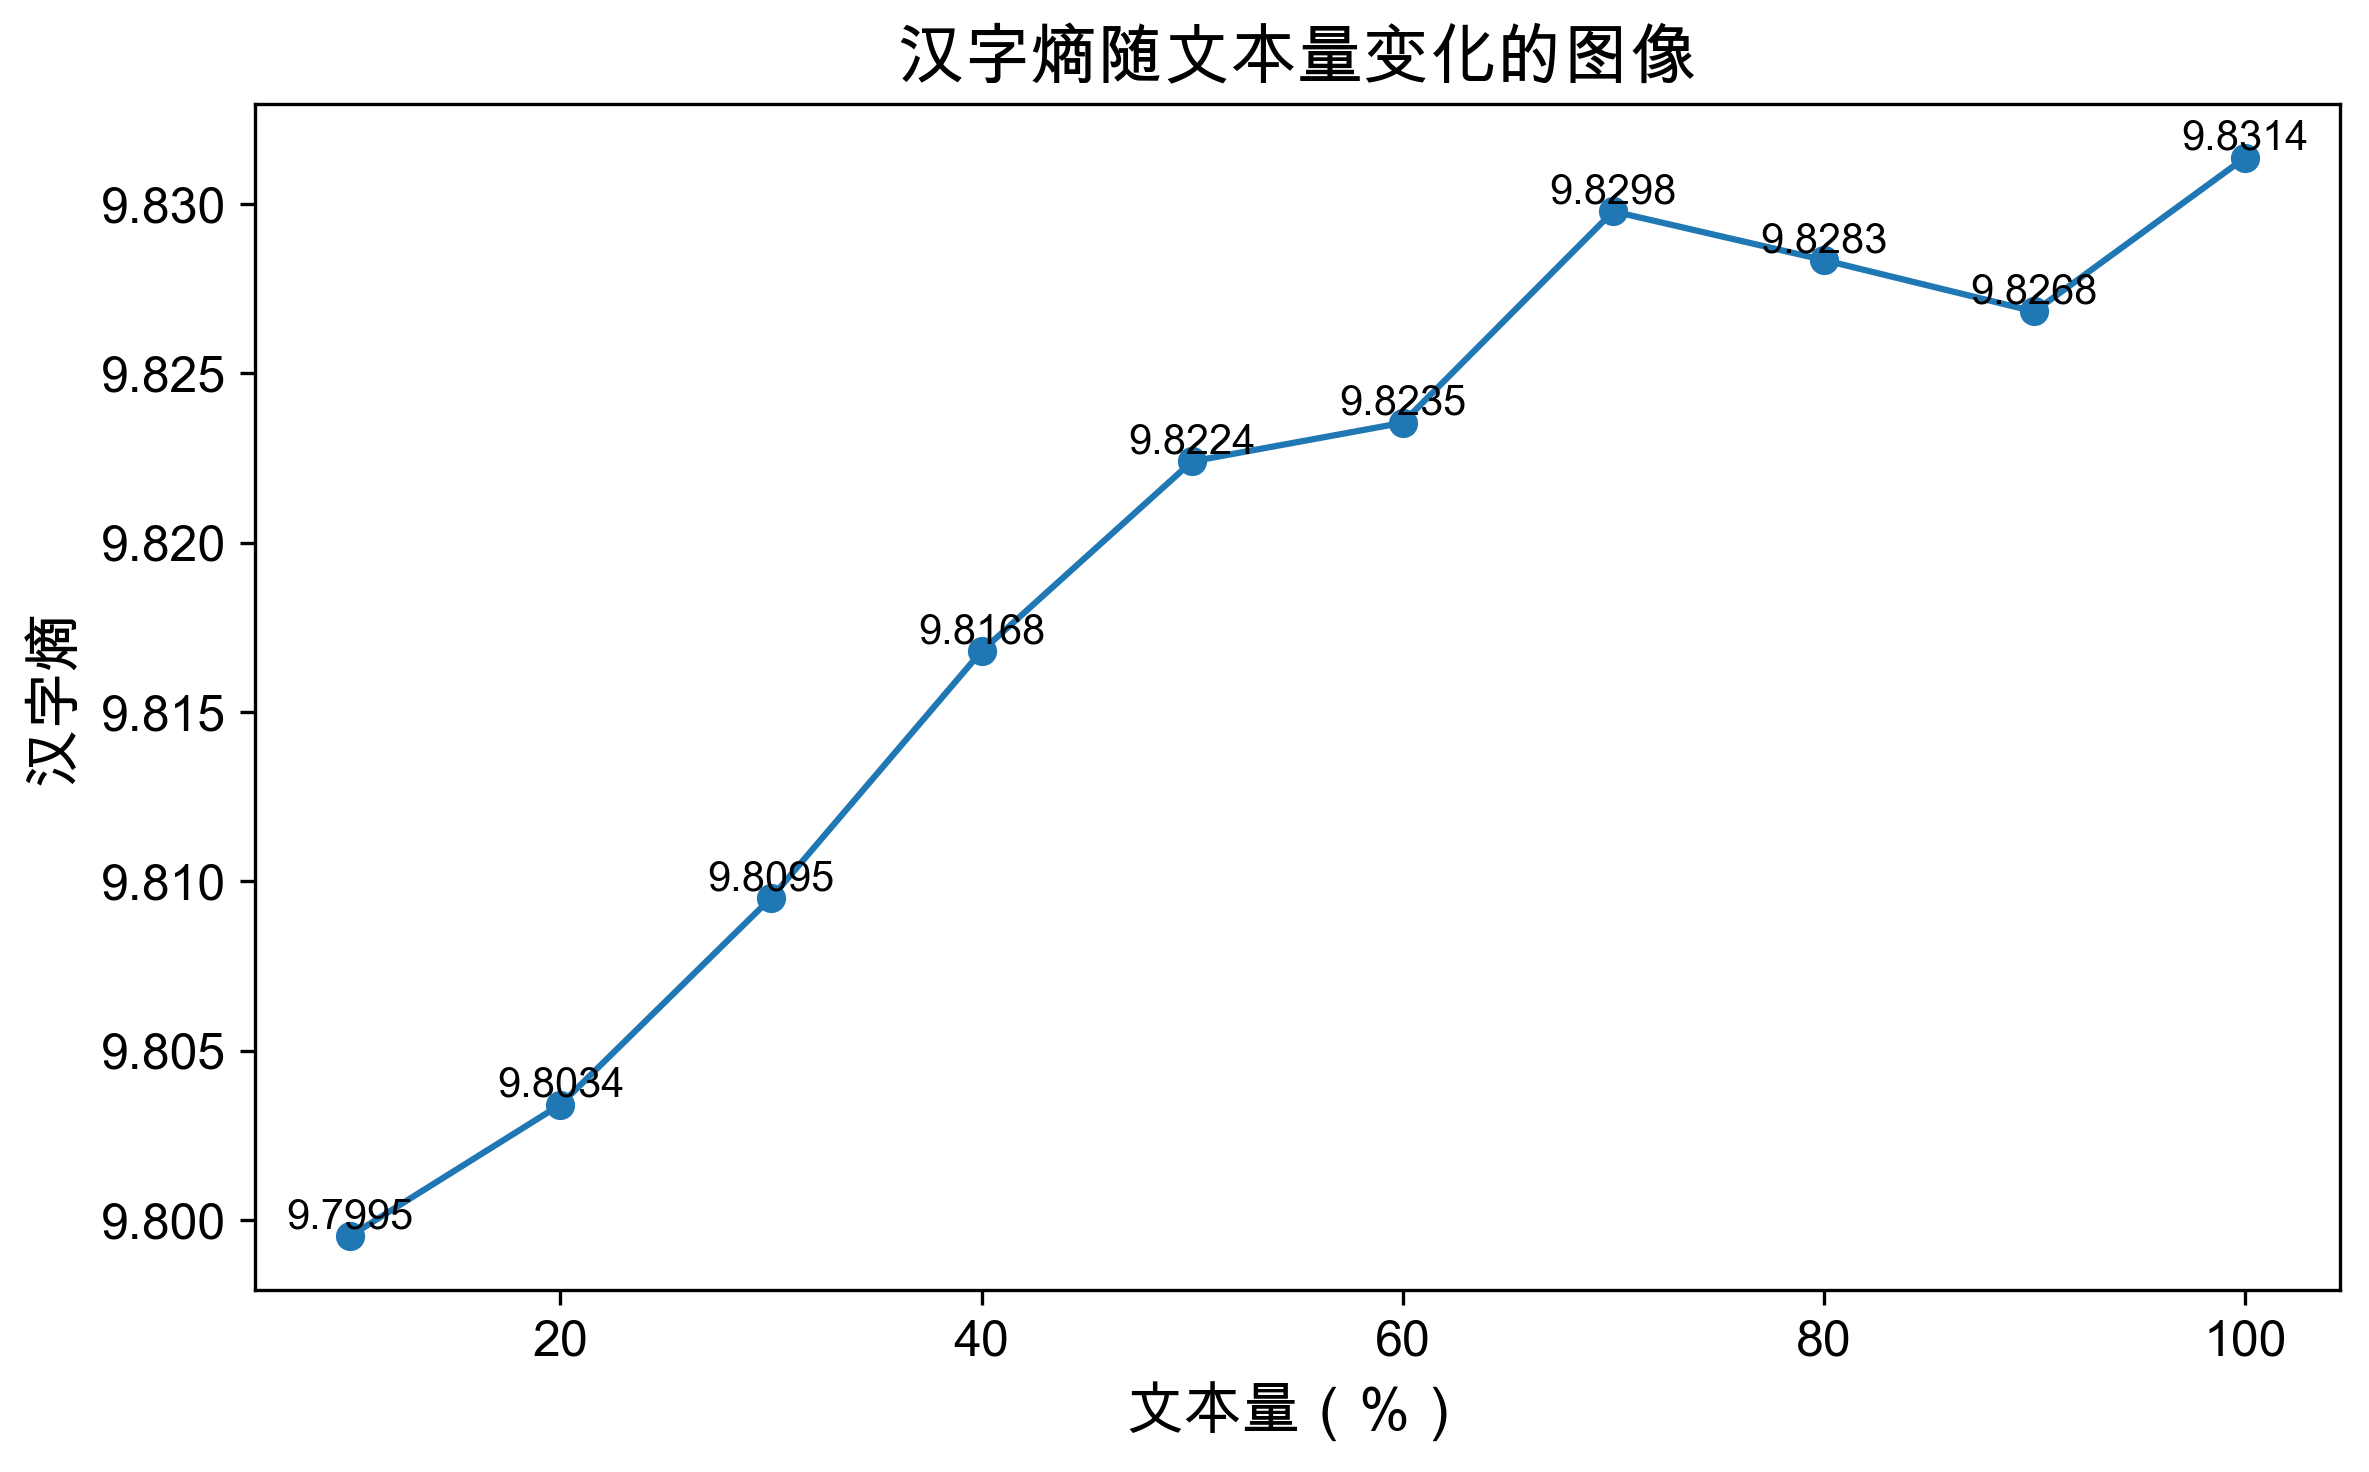
\includegraphics[width=0.7\textwidth]{zh_entropy_vs_text_size.png}
		\caption{汉字熵}
		\label{fig:3.2} 
	\end{figure}
	
	\subsection{英文分析结果}
	\subsubsection{字母}
	\subsubsection{单词}
	\subsubsection{Zipf定律}
	对于Zipf定律的验证基于英文单词的统计结果,
	
	\subsection{对比分析}
	
	\section{总结}
	\section{附录}
	\subsection{爬虫代码}
		\begin{lstlisting}[language=Python]
import requests
from bs4 import BeautifulSoup
import time
import json
import os 
import re

class TextCrawler:
	"""
	构建一个用于爬取Wikipedia随机词条的类,包括初始化、获取随机词条、爬取并保存词条等功能
	"""
	def __init__(self, lang):
		self.lang = lang
		if lang == 'zh':
			self.base_url = "https://zh.wikipedia.org/wiki/Special:Random?variant=zh-cn"    # 加上zh-cn确保爬下来的是大陆简体中文
		elif lang == 'en':
			self.base_url = "https://en.wikipedia.org/wiki/Special:Random"
		self.seen_urls = set()

	def fetch_random_article(self):
		try:
			headers = {
				'User-Agent': 'Mozilla/5.0 (Windows NT 10.0; Win64; x64) AppleWebKit/537.36 (KHTML, like Gecko) Chrome/129.0.0.0 Safari/537.36'
			}   # 添加User-Agent头
			response = requests.get(self.base_url, timeout=10, headers=headers)
			soup = BeautifulSoup(response.text, 'html.parser')
			title_tag = soup.find('title') 
			title = title_tag.text.strip()
			content_div = soup.select_one('#mw-content-text > div.mw-content-ltr.mw-parser-output')    # 直接定位到该路径
			paragraphs = content_div.find_all('p') 
			content = ''.join([p.get_text().strip() for p in paragraphs])
			content = ' '.join(content.split()) if self.lang == 'en' else re.sub(r'\s+', '', content)   # 分情况处理,英文需要用空格来分隔单词,中文直接可以把空白字符给去掉
			url = response.url
			return {'title': title, 'content': content, 'url': url} # 返回一个包含标题、内容和URL的字典,这是三个我们主要关心的内容
		except Exception as e:
			print(f"[ERROR] {self.lang} fetch failed: {e}")
			return None

	def load_existing_data(self, jsonl_path):
		"""
		加上这个是避免在程序中途中断之后,count清零,可能出现的重复爬取的情况,通过读取jsonl文件(如果存在)来确认目前已经爬取的词条数
		"""
		count = 0
		if not os.path.exists(jsonl_path): return count # 如果jsonl文件不存在说明程序第一次启动
		with open(jsonl_path, 'r', encoding='utf-8') as f:
			for line in f:
				data = json.loads(line)
				if 'url' in data:
					self.seen_urls.add(data['url'])
					count += 1
		return count

	def crawl_and_save(self, num_articles, jsonl_path):
		count = self.load_existing_data(jsonl_path)   # 从目前已经爬取的jsonl文件中确认已经爬取的词条数量
		with open(jsonl_path, 'a', encoding='utf-8') as f: 
			while count < num_articles:
				article = self.fetch_random_article()
				url = article.get('url')
				if url not in self.seen_urls:    # 通过词条的URL来判断是否重复,只要没爬过的
					self.seen_urls.add(url)
					f.write(json.dumps(article, ensure_ascii=False) + '\n')
					count += 1
				time.sleep(1)

	def crawl_both_languages(num_articles, zh_jsonl, en_jsonl):
		zh_crawler = TextCrawler('zh')
		zh_crawler.crawl_and_save(num_articles, zh_jsonl)
		en_crawler = TextCrawler('en')
		en_crawler.crawl_and_save(num_articles, en_jsonl)

if __name__ == "__main__":
	num_articles = 20000  # 每种语言爬取20000条
	crawl_both_languages(num_articles, r'HW1/zh_wikipedia.jsonl', r'HW1/en_wikipedia.jsonl')
		\end{lstlisting}
	\subsection{语料清洗代码}
		\begin{lstlisting}[language=Python]
import re
		\end{lstlisting}
	
\end{document}